\documentclass[12pt,a4paper]{article} 

\usepackage[utf8]{inputenc} % set input encoding (not needed with XeLaTeX)

%%% Examples of Article customizations
% These packages are optional, depending whether you want the features they provide.
% See the LaTeX Companion or other references for full information.


\usepackage{graphicx} % support the \includegraphics command and options
\graphicspath{ {./Figures/} }


%%% PACKAGES
\usepackage{booktabs} % for much better looking tables
\usepackage{array} % for better arrays (eg matrices) in maths
\usepackage{paralist} % very flexible & customisable lists (eg. enumerate/itemize, etc.)
\usepackage{verbatim} % adds environment for commenting out blocks of text & for better verbatim
\usepackage{subfig} % make it possible to include more than one captioned figure/table in a single float
\usepackage{pgfgantt}

% These packages are all incorporated in the memoir class to one degree or another...

%%% HEADERS & FOOTERS
\usepackage{fancyhdr} % This should be set AFTER setting up the page geometry
\pagestyle{fancy} % options: empty , plain , fancy
\renewcommand{\headrulewidth}{0pt} % customise the layout...
\lhead{}\chead{}\rhead{}
\lfoot{}\cfoot{\thepage}\rfoot{}



%%% ToC (table of contents) APPEARANCE
\usepackage[nottoc,notlof,notlot]{tocbibind} % Put the bibliography in the ToC
\usepackage[titles,subfigure]{tocloft} % Alter the style of the Table of Contents
\renewcommand{\cftsecfont}{\rmfamily\mdseries\upshape}
\renewcommand{\cftsecpagefont}{\rmfamily\mdseries\upshape} % No bold!

% ADDITIONAL PACKAGES    
\usepackage{float}
\usepackage{indentfirst} % indenting the first paragraph
\usepackage[left=2.54 cm, right=2.54 cm, top=2cm, bottom = 2 cm]{geometry} % Set page margins
\usepackage{mcite} % multiple citations
\usepackage{tocloft} % dots in table of contents
\renewcommand{\cftsecleader}{\cftdotfill{\cftdotsep}} % dots in table of contents
\usepackage{amsmath}
\usepackage{mathtools}
\usepackage[version=4]{mhchem}
\usepackage{array}
\usepackage{adjustbox}
\usepackage{tikz}
\DeclareMathOperator{\sign}{sign}
\DeclareMathOperator{\argmax}{argmax}
\DeclareMathOperator{\argmin}{argmin}
\usepackage{tikz,pgfplots}
\pgfplotsset{compat=1.18} 
\usepackage{titlesec}
\usepackage{enumitem}
\titleformat{\section}
  {\normalfont\fontsize{12}{15}\bfseries}{\thesection}{1em}{}
\usepackage[noadjust]{cite}
%%% END Article customizations



\begin{document}


\begin{center}
\textbf{MTech Project Proposal}
\end{center}

\par\noindent\rule{\textwidth}{0.5pt}

\vspace{\baselineskip}
% title
\section{Title : \textnormal{Efficient VLSI Timing Violation Screening: An Anomaly Detection Approach Using Lightweight 1D-CNNs}}

% project particulars
\section{Project Particulars}
\begin{enumerate} [label=(\Alph*)]
    \item \textbf{Project area and sub-areas:} Electronic Design Automation (EDA), Very Large Scale Integration (VLSI), Physical Design Closure, Static Timing Analysis (STA), 1-Dimensional Convolutional Neural Networks (1D-CNN), Anomaly Detection
   \item \textbf{Duration (in months):} 12 
\end{enumerate} 


% student and mentor particulars
\section{Student and Mentor Particulars}
\begin{enumerate} [label=(\Alph*)]
    \item \textbf{Student Name:} Sohang Chopra
    \item \textbf{Student Roll Number:} DA25M622
    \item \textbf{Immediate Supervisor:} Arnavesh Varun Giri
    \item \textbf{Mentor Name(s):} Arnavesh Varun Giri
\end{enumerate} 

% project summary
\section{Project Summary}

%(approximately 200 words; Overall project motivation, problem, scope, goals, and deliverables)

VLSI Physical Design is the stage in Integrated Chip Development in which logical design is converted into layout via Placement and Routing (PnR), keeping in mind the Performance, Power and Area (PPA) requirements. In this process Static Timing Analysis for timing verification has to be done repeatedly on each iteration of PnR optimization. Setup Timing Violation arises when a path fails timing verification, while Timing-Clean path is one that meets it \cite{Jenila2025A}.

Repeated timing verifications required here becomes expensive. Prominently used models are Graph Neural Networks (GNN) to improve early timing estimation, but graph construction in them requires heavy training pipeline \cite{Guo2022A,Li2025Pre-Routing}. This project proposes a lighter alternative using 1-dimensional Convolution Neural Networks (1-D CNN) for early risk screening rather than full slack regression. This is done by treating Setup Timing Violations as an anomaly detection problem, where violations are rare events among majority of the data being Timing-Clean paths.

Public OpenROAD datasets like EDA Schema V2 \cite{Shrestha2026EDA-Schema-V2:,Shrestha2024EDA-schema:} include essential information such as arrival time, slew, capacitance, etc. which we require for implementing this project. To address the heavy class imbalance (setup timing violations are rare), focal loss would be used \cite{Lin2017Focal, Mahmoodi2024Automatically} and performance would be judged by metrics such as PR-AUC (area under the curve) and F1 score.

% objectives
\section{Objectives} \label{sec:Obj}
 %List here objectives (at least 3 objectives) to solve the problem
\begin{enumerate}
\item To formulate pre-routing, post-placement setup timing violation screening as a path-level anomaly detection problem over structured sequential timing-path features derived from public OpenROAD datasets.
\item To design and implement a lightweight 1D-CNN model for early identification of likely timing-violating paths without performing full-graph slack regression.
\item To study focal-loss-based training strategies for severe class imbalance between timing-clean and timing-violating paths.
\end{enumerate}

% current state of the art
\section{Current State of The Art}

%Please provide the current state of the art related to the proposed project. This involves describing the different methods, datasets and challenges associated with the proposed project in the literature. 

Graph Neural Network (GNN) based approaches are prominent because they model circuit structure directly. A timing-engine-inspired GNN was proposed to predict arrival time and slack at timing endpoints and improved accuracy over vanilla deep GNN baselines \cite{Guo2022A}. More recent work introduced Graph Attention Network (GAT)-based timing prediction and argued that earlier GNN approaches may treat cell influences too uniformly or use overly complex delay modeling, which can limit precision and induce overfitting \cite{Li2025Pre-Routing}. These papers establish graph-based timing prediction as the current methodological reference point for this proposal.

Existing graph-based approaches are complex and have scalability and generalization limitations on large circuit graphs \cite{Li2025Pre-Routing}. This motivates exploring a lower-compute alternative when the goal is not full-chip graph reasoning, but early path-level screening of rare violations.

We frame the problem as anomaly detection, where Setup Timing Violations are rare among majority Timing-Clean paths data. 1D-CNN methods are attractive for anomaly detection of sequential data because they can directly process 1-D measurements while avoiding the larger parameter counts of 2D-CNN-style formulations \cite{Gong2022A}.

A key challenge is class imbalance. Focal loss was introduced specifically to address extreme class imbalance by down-weighting well-classified easy examples and focusing learning on hard examples \cite{Lin2017Focal}. This is directly relevant because public OpenROAD-derived datasets contain far more timing-clean than timing-violating designs and paths \cite{Shrestha2026EDA-Schema-V2:}.

% work plan
\section{Work Plan}

%Work plan describes methods and approaches to achieve the stated objectives in Section \ref{sec:Obj}. Each objective will be divided into specific work packages. Each work package may include the following: Rationale for the work-package, data science/AI algorithms to be used, experiments to be performed and rationale behind the design of experiments, and metrics to be used to evaluate different experiments, etc. 


The work will be organized into five work packages.

\textbf{WP1: Problem formulation and data specification.} The first work package will define the anomaly-screening task at path level. The target will be a binary label indicating timing-clean versus timing-violating setup paths, consistent with the proposal scope. Sequential path records will be defined from timing-related attributes available in OpenROAD-derived data, focusing on features explicitly named in the project abstract such as arrival times, slew, and capacitance. The rationale is to replace full-netlist graph prediction with a lighter path-sequence representation.

\textbf{WP2: Dataset extraction and preprocessing.} Public OpenROAD-derived datasets described in EDA-Schema-V2 will be inspected to identify the exact stage-resolved data suitable for pre-routing, post-placement timing-risk screening. Candidate designs will be selected from the publicly released benchmark suite, and path samples will be extracted, normalized, and padded or truncated to a fixed sequence format for 1D-CNN input. Because the dataset includes both timing-clean and timing-violating implementations generated by systematic parameter sweeps, it supports controlled sampling for anomaly detection experiments \cite{Shrestha2026EDA-Schema-V2:}.

\textbf{WP3: Lightweight 1D-CNN design.} A compact 1D-CNN classifier will be implemented for binary anomaly screening. The design rationale is that 1D-CNNs are well suited to raw or structured 1-D sequential inputs and can reduce parameter count relative to heavier alternatives \cite{Gong2022A}. The model will remain intentionally lightweight so that training and inference are feasible on consumer hardware.

\textbf{WP4: Imbalance-aware training and evaluation.} Training will compare standard binary cross-entropy against focal-loss-based objectives. The rationale is that focal loss reduces domination by easy majority examples and emphasizes hard minority cases \cite{Lin2017Focal}. Experiments will evaluate PR-AUC and F1-score as primary metrics, since the target class is rare. Precision, recall, confusion matrix, and training/inference time will be collected as supporting metrics.

\textbf{WP5: Baseline comparison and resource study.} The final work package will compare the proposed method against literature-reported graph-based timing predictors qualitatively on task formulation and quantitatively on screening performance and computational footprint where feasible. Because recent GNN timing systems use deeper graph models and stronger hardware \cite{Ding2024A}, this package will emphasize efficiency-oriented comparison: model size, memory demand, CPU feasibility, and optional low-cost GPU usage.

\section{Data Sets}

%Please provide description of data sets to be used in this project. Do you have data sets with you or is the data in the public domain? If the data will be generated by you via a set of simulations, please provide details of how will you generate the data, choice of experimental conditions for the generation of the data, how will you ensure that the experiments emulate the real-world scenario. If you are using an industrial data set (which cannot be shared), the performance of different methods and/or proposed solution(s) in the thesis must be provided in relative terms along with appropriate masking. If you are using data from the public domain, provide the link. 

This project is planned around public-domain data from the OpenROAD ecosystem. The primary intended source is the EDA-Schema-V2 dataset. The dataset contains approximately 7,800 design instances across 18 benchmark circuits, stage-resolved representations from synthesis through detailed routing, and more than 36 million extracted timing paths. Importantly for this proposal, the dataset captures both timing-clean and timing-violating implementations generated through systematic sweeps of clock period, core utilization, and aspect ratio \cite{Shrestha2026EDA-Schema-V2:}.

The public dataset link to EDA Schema V2 is https://github.com/drexel-ice/EDA-schema .

\section{Expected deliverables/outcomes}

%Please provide 4-5 bullet points describing the expected outcome(s) of this project that can be quantitatively measured at the end of the project. 

\begin{itemize}
\item A lightweight 1D-CNN implementation for binary screening of timing-clean versus timing-violating paths.
\item Quantitative evaluation of the proposed model using PR-AUC, F1-score, precision, and recall.
\item Quantitative comparison of focal loss versus standard loss functions under severe class imbalance.
\item A resource-efficiency report covering model size, training time, inference time, and feasibility on personal low-cost hardware.
\end{itemize}

\section{Significance of the expected outcome(s) with respect to the state-of-the-art in 
the field}

%Discuss the impact of the expected project outcome(s) on the current state of knowledge in the field.

The state-of-the-art in the field is primarily graph-based neural network approaches. As these are heavy, this project aims to produce lightweight 1-D CNN model for early screening of rare violating paths which would provide a public-data baseline. it explores whether a lightweight 1D-CNN can provide acceptable screening performance under hardware constraints similar to those of individual researchers. This would complement, rather than replace, existing GNN-based timing-prediction research.

\section{Implementation arrangements proposed for the project (linkages and management structure) }

% Provide a plan of action for implementing the project. For example, what is the plan to collect relevant data, gain requisite domain knowledge (if required), etc.

The project will be implemented in a staged manner. First, domain knowledge will be consolidated from OpenROAD flow papers and timing-prediction literature to define the exact meaning of setup slack, violating paths, and stage-specific timing context \cite{Ajayi2019INVITED:,Kahng2021The,Li2025Pre-Routing}. Second, public OpenROAD-derived datasets will be obtained and inspected to identify the exact files, schema fields, and timing-path representations needed for the proposed binary screening setup \cite{Shrestha2026EDA-Schema-V2:,Shrestha2024EDA-schema:}. Third, a preprocessing pipeline will be built for sequence extraction, label assignment, normalization, and dataset splitting. Fourth, the lightweight 1D-CNN and focal-loss training pipeline will be implemented in a standard deep-learning framework. Finally, experiments and ablations will be run, documented, and summarized in reproducible scripts and result tables.

As mentioned, data is available in public dataset link shared previously. I would be executing data preparation, model development, and experiments, with periodic review by my project mentor.

\section{Resource Requirements and their availability}

%Software and hardware requirements and their availability should be listed here.

\textbf{Software:} Python, PyTorch, common scientific-computing libraries, and data-processing tools are required. These software components are open source and publicly accessible.

\textbf{Hardware:} The project is intended to be feasible on a laptop and cloud notebook GPUs for data preparation, preprocessing, experiments, and baseline model development.


\section{Risks}

%What are the risks involved in the project from the completion perspective ?

The exact publicly available timing-path fields may require additional preprocessing effort before they match the intended sequential input format, and class imbalances would need to be handled. A lightweight model may trade off predictive power against efficiency and therefore may underperform graph-based approaches on absolute accuracy. These risks are manageable because the project goal is to establish an efficient baseline rather than to claim state-of-the-art accuracy.


\section{Gantt chart}  

%Provide a timeline and milestones for each work package using a Gantt Chart. An example is given in Figure \ref{fig:ganntex}.

Work timeline and milestones are shown for each work package using a Gantt Chart (months are numbered 1 to 12):

\begin{figure}[h!]
    \centering
    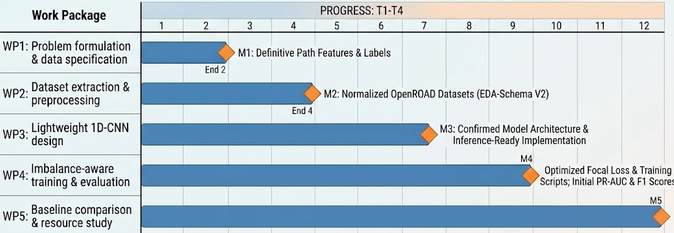
\includegraphics[width=0.85\textwidth]{Figures/gantt_chart_proposal.png}
    \caption{Project Timeline}
    \label{fig:ganntex}
\end{figure}

\pagebreak

\bibliographystyle{IEEEtran}
\bibliography{reflist}

\end{document}